\section{\lr{Vector Processing}}
\begin{enumerate}
    \item سعی کردم که در کد کامنت‌هایی قرار دهم که فهم آن راحت‌تر شود:
    \codesample{codes/3-a.s}
    پس برای حساب کردن تعداد کلاک‌ها در ابتدا حساب می‌کنیم که قسمت
    \lr{initialize}
    کردن کد چه قدر زمان می‌برد.
    \begin{gather*}
        1 + 4 \times 1 = 5
    \end{gather*}
    حال هر حلقه‌ی
    \lr{loop}
    را حساب می‌کنیم.
    \begin{gather*}
        11 + 11 + 6 + 11 + 4 + 1 + 11 + 4 + 1 = 60
    \end{gather*}
    در مجموع نیز ۱۰۰ بار این حلقه اجرا می‌شود پس در نهایت داریم:
    \begin{gather*}
        60 \times 100 + 5 = 6005
    \end{gather*}
    \item کد را به صورت زیر می‌نویسیم: (فرض می‌کنیم که جمع آدرس با عدد ثابت در مرحله‌ی \lr{decode} انجام می‌شود.)
    \codesample{codes/3-b.s}
    برای محاسبه مشخص است که در ابتدا دو دستور \lr{SET} تنها دو کلاک را از ما می‌گیرند.
    بقیه‌ی دستورات را نیز در زیر آوردام که چه قدر طول می‌کشند.
    همچنین فرض می‌کنیم تعداد بانک‌های حافظه حداقل 11 است.
    \begin{gather*}
        \underbrace{1 + 1}_{\text{\lr{SET}}} + \underbrace{11 + 63}_{\text{\lr{VLD, V0, B}}} + \underbrace{11 + 63}_{\text{\lr{VLD, V1, C}}} + \underbrace{6 + 63}_{\text{\lr{VMUL V0, V0, V1}}} + \underbrace{11 + 63}_{\text{\lr{VLD V1, D}}} + \underbrace{4 + 63}_{\text{\lr{VADD V0, V0, V1}}} + \underbrace{1 + 63}_{\text{\lr{VRSHFA}}} + \underbrace{11 + 63}_{\text{\lr{VST V0, A}}} \\
        = 498
    \end{gather*}
    برای قسمت دوم کد نیز به صورت مشابه داریم:
    \begin{gather*}
        \underbrace{1}_{\text{\lr{SET}}} + \underbrace{11 + 35}_{\text{\lr{VLD, V0, B}}} + \underbrace{11 + 35}_{\text{\lr{VLD, V1, C}}} + \underbrace{6 + 35}_{\text{\lr{VMUL V0, V0, V1}}} + \underbrace{11 + 35}_{\text{\lr{VLD V1, D}}} + \underbrace{4 + 35}_{\text{\lr{VADD V0, V0, V1}}} + \underbrace{1 + 35}_{\text{\lr{VRSHFA}}} + \underbrace{11 + 35}_{\text{\lr{VST V0, A}}} \\
        = 290
    \end{gather*}
    پس در نهایت
    $498 + 290 = 788$
    کلاک زمان می‌برد.
    \item در این حالت عملا زمان خواندن از مموری درجا می‌توان داده را به \lr{ALU} داد.
    سپس شکلی مانند اسلاید‌های درس کشیدم:
    \begin{figure}[H]
        \centering
        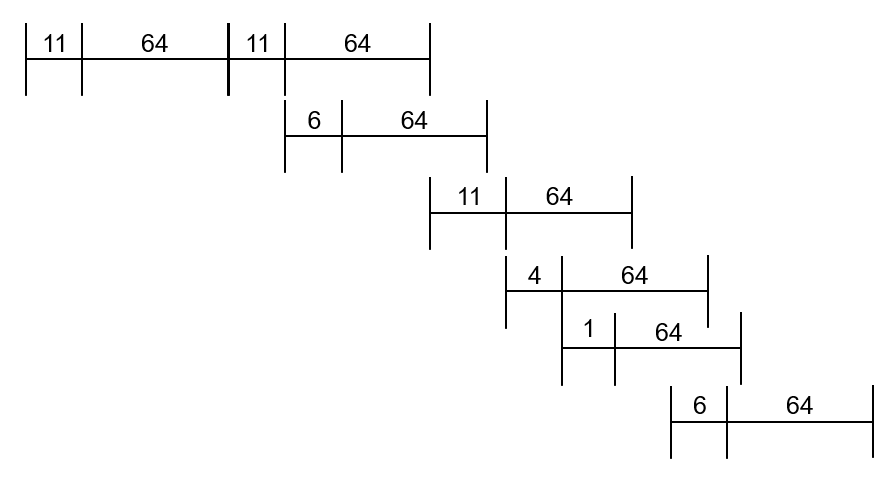
\includegraphics[scale=0.45]{pics/3-c.png}
    \end{figure}
    یک نکته‌ی مهم که وجود دارد این است که
    \lr{store}
    آخر باید بعد از زمانی اتفاق بیفتد که آخرین لود تمام شده باشد چرا که مموری ما امکان پشتیبانی از یک
    \lr{load} و \lr{store}
    موازی را ندارد. دقت کنید که این موضوع برای لود سوم نیز صادق است.
    با کمی فکر کردن متوجه می‌شویم که این کار عملا مثل چهار لود پشت سر هم است!
    پس برای حساب کردن زمان اجرا داریم:
    \begin{gather*}
        4 \times (11 + 63) = 296
    \end{gather*}
    به صورت مشابه برای قسمت دوم نیز داریم:
    \begin{gather*}
        4 \times (11 + 35) = 184
    \end{gather*}
    پس در کل
    $296 + 184 = 480$
    سیکل طول می‌کشد.
\end{enumerate}